\documentclass[a4paper,14pt]{extarticle}

\usepackage[utf8x]{inputenc}
\usepackage[T1,T2A]{fontenc}
\usepackage[russian]{babel}
\usepackage{hyperref}
\usepackage{indentfirst}
\usepackage{here}
\usepackage{array}
\usepackage{graphicx}
\usepackage{caption}
\usepackage{subcaption}
\usepackage{chngcntr}
\usepackage{amsmath}
\usepackage{amssymb}
\usepackage{pgfplots}
\usepackage{pgfplotstable}
\usepackage[left=2cm,right=2cm,top=2cm,bottom=2cm,bindingoffset=0cm]{geometry}
\usepackage{multicol}
\usepackage{askmaps}
\usepackage{enumitem}

\setitemize{itemsep=0em}
\setenumerate{itemsep=0em}

\renewcommand{\le}{\ensuremath{\leqslant}}
\renewcommand{\leq}{\ensuremath{\leqslant}}
\renewcommand{\ge}{\ensuremath{\geqslant}}
\renewcommand{\geq}{\ensuremath{\geqslant}}
\renewcommand{\epsilon}{\ensuremath{\varepsilon}}
\renewcommand{\phi}{\ensuremath{\varphi}}
\renewcommand{\thefigure}{\arabic{figure}} 	
\renewcommand*\not[1]{\overline{#1}}

%\titleformat*{\section}{\large\bfseries} 
%\titleformat*{\subsection}{\normalsize\bfseries} 
%\titleformat*{\subsubsection}{\normalsize\bfseries} 
%\titleformat*{\paragraph}{\normalsize\bfseries} 
%\titleformat*{\subparagraph}{\normalsize\bfseries} 

\counterwithin{figure}{section}
\counterwithin{equation}{section}
\counterwithin{table}{section}
\newcommand{\sign}[1][5cm]{\makebox[#1]{\hrulefill}}
\graphicspath{{../pics/}}
\captionsetup{justification=centering,margin=1cm}
\def\arraystretch{1.3}
\setlength\parindent{5ex}
%\titlelabel{\thetitle.\quad}

\begin{document}

\begin{titlepage}
\begin{center}
	Санкт-Петербургский Политехнический Университет Петра Великого\\[0.3cm]
	Институт компьютерных наук и технологий \\[0.3cm]
	Кафедра компьютерных систем и программных технологий\\[4cm]
	
	\textbf{ОТЧЕТ}\\ 
	\textbf{по лабораторной работе}\\[0.5cm]
	\textbf{<<Исследование персептронов>>}\\[0.1cm]
	\textbf{Нейроинформатика}\\[4.0cm]
\end{center}

\begin{flushright}
	\begin{minipage}{0.45\textwidth}
		\textbf{Работу выполнил студент}\\[3mm]
		группа 33501/4 \hspace*{10mm} Дьячков В.В.\\[5mm]
		\textbf{Преподаватель}\\[5mm]
		\sign[1.7cm] \hspace*{1mm} к.т.н., доц. Никитин К.В. \\[5mm]
	\end{minipage}
\end{flushright}

\vfill

\begin{center}
	Санкт-Петербург\\
	\the\year
\end{center}
\end{titlepage}

\addtocounter{page}{1}

\tableofcontents
\newpage
\listoftables
\listoffigures
\newpage

\section{Цели работы}

\begin{itemize}
	\item Приобретение навыков построения, инициализации и обучения РФБ-НС.
	\item Исследование РФБ-НС при решении задач аппроксимации статических зависимостей и классификации.
\end{itemize}

\section{Аппроксимация статических зависимостей}

\subsection{Формирование обучающей и тестовой выборки}

%Задайте достаточное для точной аппроксимации количество обучающих примеров (в данном случае совпадающее с числом РБФ-нейронов).

Сформируем обучающую и тестовую выборки на основе ранее созданных функций. На рис. \ref{fig:2_1} изображены сформированные выборки. Исходная выборка из $100$ примеров была разделена на обучающую и тестовую в соотношении $0.7 : 0.3$.

\begin{figure}[H]
\begin{center}
	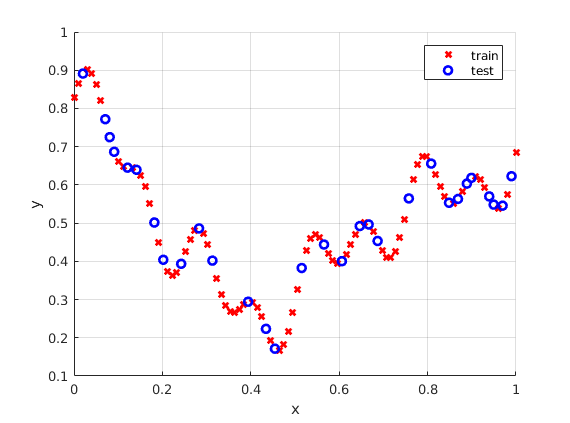
\includegraphics[scale=0.9]{2_1}
	\caption{Обучающая и тестовая выборки}
	\label{fig:2_1}
\end{center}
\end{figure}

\subsection{Аппроксимация с помощью точной РБФ-НС}

%Изменяя ширину РБФ (spread), определите наилучшее значение этого параметра с точки зрения качества аппроксимации. Постройте три графика аппроксимации для разных значений spread: оптимального, больше и меньше оптимального, когда явно видно, что аппроксимация плохая. При построении графиков аппроксимации не забывайте приводить графики исходной желаемой зависимости.
%Постройте график зависимости ошибки аппроксимации от параметра spread в логарифмическом масштабе.
%С помощью точной РБФ-НС (newrbe) аппроксимируйте функцию (для вашего варианта из заданий с номером 5).

Подберем наилучшее значение параметра \code{spread} для обучения с помощью точной РБФ-НС. На рис. \ref{fig:2_2_1} изображена зависимость ошибки \code{perform} от значения параметра \code{spread} в логарифмическом масштабе. 
\begin{figure}[H]
\begin{center}
	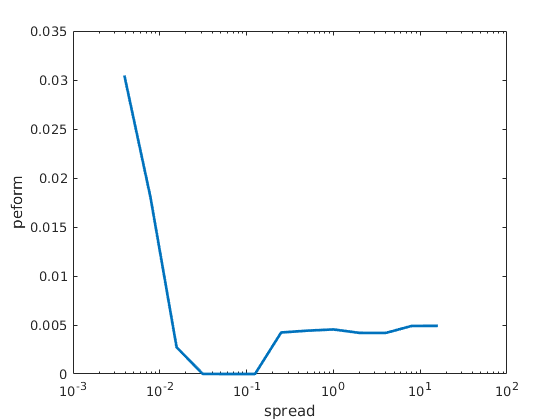
\includegraphics[scale=0.9]{2_2_1}
	\caption{Зависимость \code{perform} от \code{spread}}
	\label{fig:2_2_1}
\end{center}
\end{figure}

Оптимальным можно считать значения \code{spread} $\leq 0.1$. Постром два графика аппроксимации для оптимального значения \code{spread} и больше оптимального. При уменьшении параметра даже до $10^{-10}$ функция аппроксимируется без ошибок. На рис. \ref{fig:2_2_2} изображены построенные аппроксимации.
\begin{figure}[H]
\begin{center}
	\begin{subfigure}{0.49\textwidth}
		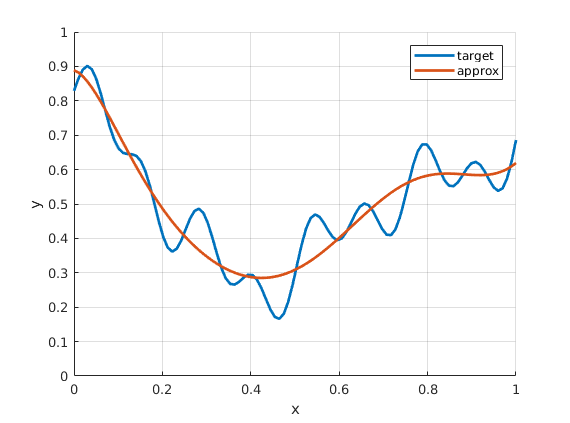
\includegraphics[width=\textwidth]{2_2_2}
		\caption{\code{spread = 1}}
	\end{subfigure}
	\begin{subfigure}{0.49\textwidth}
		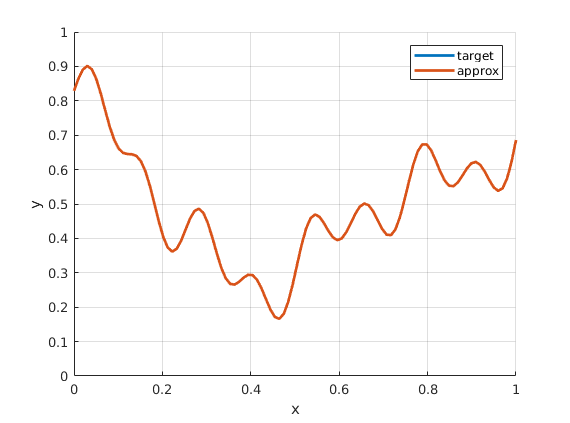
\includegraphics[width=\textwidth]{2_2_3}
		\caption{\code{spread = 0.1}}
	\end{subfigure}
	\caption{Аппроксимация при разных значениях \code{spread}}
	\label{fig:2_2_2}
\end{center}
\end{figure}

\subsection{Аппроксимация с помощью приближенной РБФ-НС}

%Изменяя значение допустимой ошибки (goal), постройте зависимость числа используемых РБФ-нейронов от допустимой ошибки аппроксимации. Для промежуточных результатов постройте графики аппроксимации.

На рис. \ref{fig:2_3_1} изображена зависимость числа используемых РБФ-нейронов от допустимой ошибки аппроксимации \code{goal} в логарифмическом масштабе.
\begin{figure}[H]
\begin{center}
	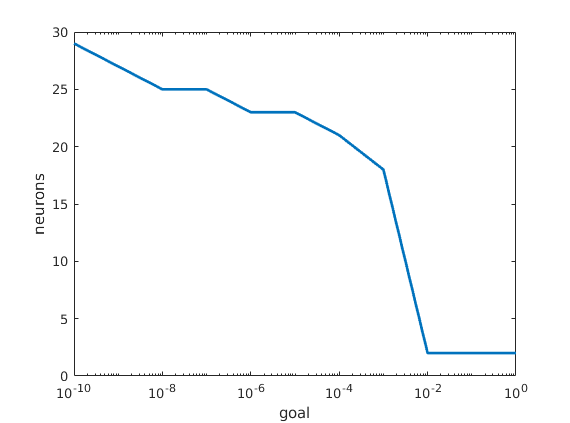
\includegraphics[scale=0.9]{2_3_1}
	\caption{Зависимость числа нейронов от \code{goal}}
	\label{fig:2_3_1}
\end{center}
\end{figure}

На рис. \ref{fig:2_3_2} изображены аппроксимации при разных значениях допустимой ошибки.
\begin{figure}[H]
\begin{center}
	\begin{subfigure}{0.49\textwidth}
		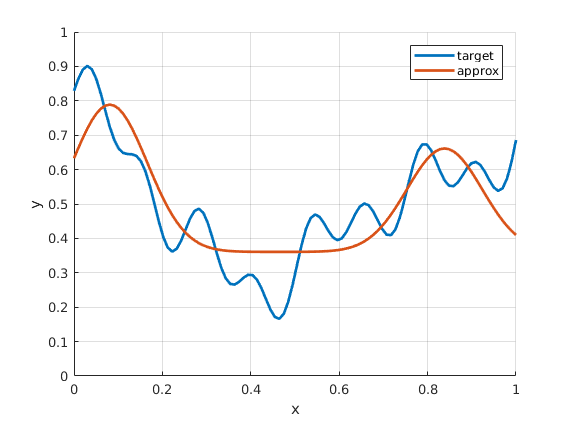
\includegraphics[width=\textwidth]{2_3_2}
		\caption{\code{goal = 0.01} (2 нейрона)}
	\end{subfigure}
	\begin{subfigure}{0.49\textwidth}
		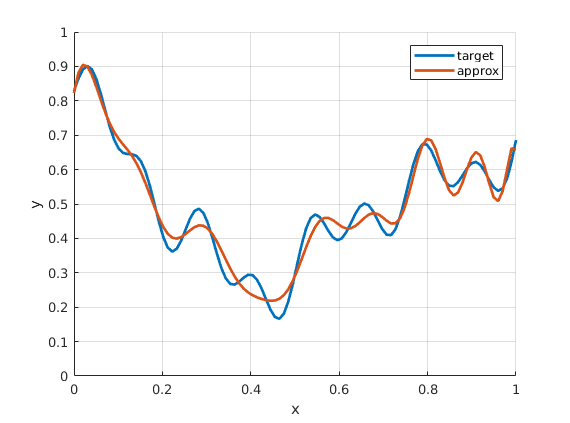
\includegraphics[width=\textwidth]{2_3_3}
		\caption{\code{goal = 0.001} (18 нейронов)}
	\end{subfigure}
	\begin{subfigure}{0.49\textwidth}
		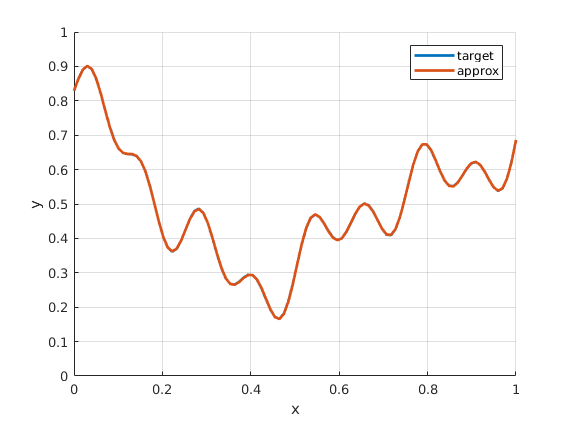
\includegraphics[width=\textwidth]{2_3_4}
		\caption{\code{goal = 0.0001} (23 нейрона)}
	\end{subfigure}
	\caption{Аппроксимация при разных значениях \code{goal}}
	\label{fig:2_3_2}
\end{center}
\end{figure}

\subsection{Аппроксимация с помощью GRNN}

%По аналогии с newrb изменяя ширину РБФ (spread), определите наилучшее значение этого параметра с точки зрения качества аппроксимации. Постройте график аппроксимации на исходной зависимости.
%Уменьшите объем обучающей выборки в несколько раз (рассмотрите 3 случая) и подберите оптимальные значения параметра spread для каждого случая. Постройте полученные графики аппроксимации. Приведите значения ошибок.

Подберем наилучшее значение параметра \code{spread} для обучения с помощью GRNN. На рис. \ref{fig:2_4_1} изображена зависимость ошибки \code{perform} от значения параметра \code{spread} в логарифмическом масштабе. 
\begin{figure}[H]
\begin{center}
	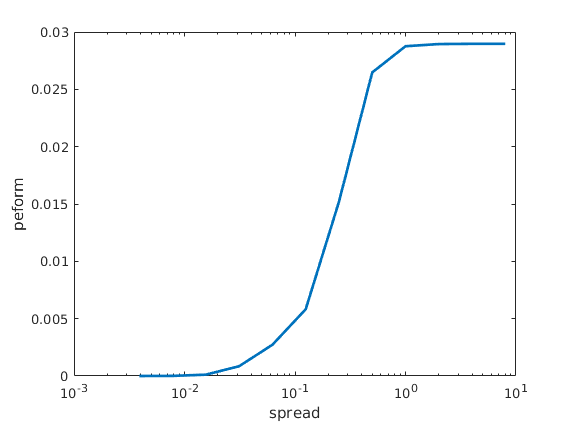
\includegraphics[scale=0.9]{2_4_1}
	\caption{Зависимость \code{perform} от \code{spread}}
	\label{fig:2_4_1}
\end{center}
\end{figure}

Оптимальным можно считать значения \code{spread} $\leq 0.01$. Постром два графика аппроксимации для оптимального значения \code{spread} и больше оптимального. При уменьшении параметра даже до $10^{-10}$ функция аппроксимируется без ошибок. На рис. \ref{fig:2_4_2} изображены построенные аппроксимации.
\begin{figure}[H]
\begin{center}
	\begin{subfigure}{0.49\textwidth}
		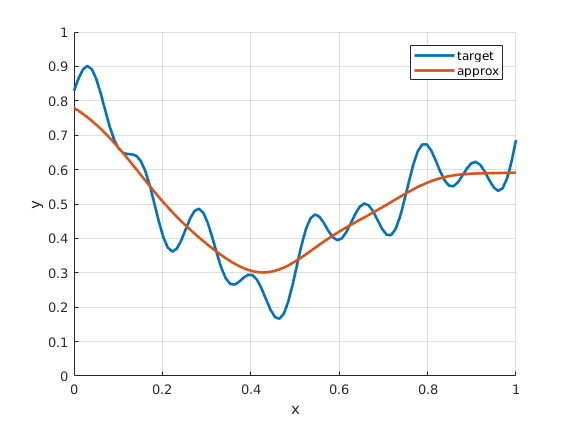
\includegraphics[width=\textwidth]{2_4_2}
		\caption{\code{spread = 0.1}}
	\end{subfigure}
	\begin{subfigure}{0.49\textwidth}
		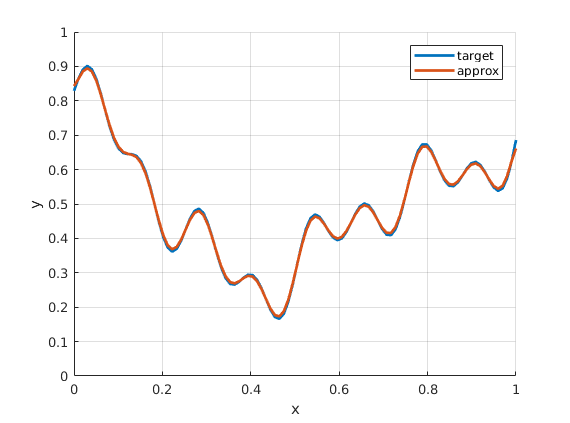
\includegraphics[width=\textwidth]{2_4_3}
		\caption{\code{spread = 0.01}}
	\end{subfigure}
	\caption{Аппроксимация при разных значениях \code{spread}}
	\label{fig:2_4_2}
\end{center}
\end{figure}

\subsection{Сравнение качества апрпоксимации}

%Сравните качество аппроксимации сетями прямого распространения и различными вариантами РБФ-НС (точной, приближенной РБФ-НС и GRNN) по различным показателям:
%- число нейронов, требуемое для достижения заданного качества аппроксимации;
%- время обучения;
%- сложность настройки (выбора параметров) НС.
%Постройте на одном графике зависимости ошибки от числа нейронов для различных типов НС.

\newpage

\section{Разбиение плоскости на $2$ класса}

\subsection{Формирование обучающей и тестовой выборки}

%Задайте достаточное для точной классификации количество обучающих примеров.

Сформируем обучающую и тестовую выборки на основе ранее созданных функций. На рис. \ref{fig:3_1} изображены сформированные выборки.
\begin{figure}[H]
\begin{center}
	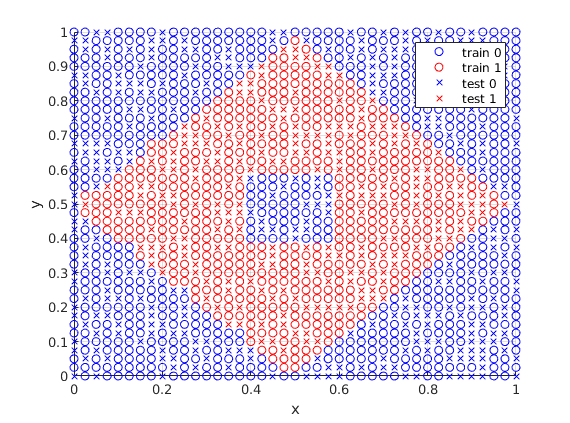
\includegraphics[scale=1]{3_1}
	\caption{Обучающая и тестовая выборки}
	\label{fig:3_1}
\end{center}
\end{figure}

\subsection{Подбор значения spread}

%Подберите оптимальное значение spread в смысле минимальной ошибки на тестовой выборке. Визуализируйте результаты классификации (диаграмма соотнесения тестовых примеров с классами, раскраска плоскости). Приведите значение средней ошибки.
%Постройте дополнительно графики классификации для значений spread, больших и меньших оптимального, когда явно видно, что классификация неудовлетворительная.

\subsection{Уменьшение объема выборки}

%Уменьшите объем обучающей выборки в несколько раз (рассмотрите 3 случая) и подберите оптимальные значения параметра spread для каждого случая. Визуализируйте результаты классификации и приведите значение средней ошибки.

\subsection{Сравнение качества классификации}

%Постройте поверхность ошибки в плоскости двух параметров: ширина РБФ-функции spread и объем обучающей выборки.
%Сравните полученные результаты с НС прямого распространения по аналогии с п. 3 задания 1.

\newpage

\section{Разбиение плоскости на $N$ классов}

\subsection{Формирование обучающей и тестовой выборки}

Сформируем обучающую и тестовую выборки на основе ранее созданных функций. На рис. \ref{fig:4_1} изображены сформированные выборки: обучающая выборка обозначена ноликами, а тестовая -- крестиками.
\begin{figure}[H]
\begin{center}
	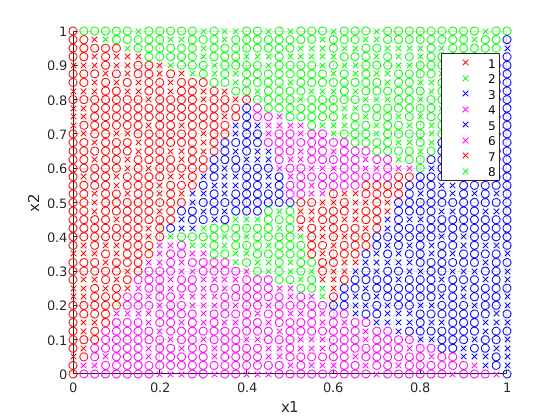
\includegraphics[scale=1]{4_1}
	\caption{Обучающая и тестовая выборки}
	\label{fig:4_1}
\end{center}
\end{figure}

\subsection{Подбор значения spread}

%Подберите оптимальное значение spread в смысле минимальной ошибки на тестовой выборке. Визуализируйте результаты классификации (диаграмма соотнесения тестовых примеров с классами, раскраска плоскости). Приведите значение средней ошибки.
%Постройте дополнительно графики классификации для значений spread, больших и меньших оптимального, когда явно видно, что классификация неудовлетворительная.
%Дополнительно приведите матрицы неточностей и рассчитайте ошибки первого и второго родов.

\subsection{Уменьшение объема выборки}

%Уменьшите объем обучающей выборки в несколько раз (рассмотрите 3 случая) и подберите оптимальные значения параметра spread для каждого случая. Визуализируйте результаты классификации и приведите значение средней ошибки.

\subsection{Сравнение качества классификации}

%Постройте поверхность ошибки в плоскости двух параметров: ширина РБФ-функции spread и объем обучающей выборки.
%Сравните полученные результаты с НС прямого распространения по аналогии с п. 3 задания 1.

\newpage

\section{Классификация многомерных образов}

\subsection{Формирование обучающей и тестовой выборки}

%Сформируйте обучающую выборку достаточного объема.

На рис. \ref{fig:5_1} изображены примеры обучающих и тестовых образов.
\begin{figure}[H]
\begin{center}
	%\includegraphics[scale=1]{5_1}
	\caption{Примеры обучающей и тестовай выборки}
	\label{fig:5_1}
\end{center}
\end{figure}

\subsection{Подбор значения spread}

%Подберите оптимальное значение spread.

\subsection{Качество классификации}

%Исследуйте качество классификации на тестовой выборке, содержащей зашумленные примеры. Приведите матрицу неточностей, рассчитайте среднюю ошибку и ошибки 1,2 родов.

\subsection{Изменение объема выборки}

%Попробуйте увеличить и уменьшить объем обучающей выборки в несколько раз. Для каждого случая подберите оптимальное значение spread и рассчитайте показатели качества классификации.
%Проанализируйте полученные результаты, сравнив их с результатами классификации тех же самых образов НС прямого распространения по аналогии с п. 3 задания 1.

\section{Выводы}

В данной работе были приобретены навыки построения, инициализации и обучения нейронных сетей с радиально-базисными функциями для решения задач аппроксимации статической аппроксимации и классификации. Были изучены точные РБФ-НС, приближенные РБФ-НС и GRNN.

\end{document}